\chapter{Contraction Hierarchies, Hierarchical Hub Labelings}\label{chapter:ch}

Mit dem Aufkommen von Online-Kartendiensten stieg der Bedarf an effizienten Algorithmen zur Berechnung kürzester Pfade in großen Netzwerken stark an.
\cite{geisberger2008contraction} stellte hierfür \emph{Contraction Hierarchies} vor.
Diese Methode nutzt ein ähnliches Konzept wie die in \autoref{graphs:strassengraphen} vorgestellte Idee der Wichtigkeit von Kanten und ermöglicht auf Straßengraphen einen Speedup um mehrere Größenordnungen.
Darauf aufbauend stellte \cite{abraham2011hub} eine Methode (\emph{Hierarchical Hub Labelings}) vor, welche einen mit \emph{Contraction Hierarchies} bearbeiteten Graphen als Eingabe erwartet und noch einmal einen Speedup um einige Größenordnungen ermöglicht.
In diesen Kapitel werden die Grundlagen dieser Ansätze erläutert, und im \autoref{chapter:kontraktion} wird die Anwendbarkeit dieser Methoden auf Sichtbarkeitsgraphen diskutiert.

\section{Contraction Hierarchies}

Die Grundidee der Contraction Hierarchies ist es, aus einem Graph zwei Graphen zu erzeugen, in denen die Suche nur einen kleinen Teil aller Knoten betrachtet, wodurch das Suchen in ihnen deutlich effizienter ist.
Durch die spezielle Konstruktion dieser Graphen ist garantiert, dass die Suche vom Startknoten aus in dem einen und die Suche vom Zielknoten aus in dem anderen Graphen immer einen Knoten findet, der auf dem kürzesten Pfad zwischen dem Startknoten und dem Zielknoten liegt.
Der kürzeste Pfad kann dann, wie bei einer bidirektionalen Dijkstra-Suche, aus den Teilsuchen erstellt werden.

Während der Vorbereitsungphase werden nacheinander alle Knoten das Graphens \emph{kontrahiert}, wobei für die jeweils übrigen Knoten die kürzeste Pfad Distanz erhalten bleibt.
Nachtdem alle Knoten kontrahiert wurden, werden die erwähnten beiden Graphen gebaut, auf denen dann gesucht werden kann.

\subsection{Knoten-Kontraktion}

Der Name Contraction Hierarchies leitet sich aus dem Konzept der Knoten-Kontraktion (Contraction) ab.

\begin{definition}[Knoten-Kontraktion]
  Sei $G = (V, E)$ ein Graph. Sei $v \in V$ der zu kontrahierende Knoten. Die Kontraktion von $v$ erfolgt in zwei Schritten:

  \begin{enumerate}
    \item\label{ch:contraction:when_shortcut}
      Für jeden Vorgänger $u \in V$ und jeden Nachfolger $w \in V$ von $v$ wird, wenn $v$ auf allen kürzesten Pfaden zwischen $u$ und $w$ liegt, eine Abkürzungskante (Shortcut) $(u, w, {spd}_G((u, w)))$ zu $E$ hinzugefügt.

    \item
      Alle Kanten von und zu $v$ werden entfernt.
  \end{enumerate}
\end{definition}

Nach der Kontraktion $v$ ist also isoliert.
Um die Abkürzungen zu erzeugen, kann von jedem Vorgänger eine modifizierte Dijkstra-Suche zu allen Nachfolgern ausgeführt werden, bei der die Kanten von und zu $v$ nicht begangen werden.
Ist die Länge der potenziellen Abkürzung kürzer, als die des in der modifizierten Dijkstra-Suche gefundenen Pfades, so liegt $v$ auf allen kürzesten Pfaden zwischen $u$ und $w$.
Die Knoten-Kontraktion bewahrt daher die kürzesten Pfad Distanzen zwischen den verbleibenden Knoten.

\todo{
  wenn $v$ auf allen kürzesten Pfaden zwischen $u$ und $w$ liegt

  Beispiele
}

Betrachten wir dies am ungerichteten Beispielgraphen.
Sei $i$ der zu kontrahierende Knoten, die Nachbarn sind $a$, $b$, $j$ und $h$.
Die kürzesten $a$-$b$-, $b$-$j$-, $h$-$j$- und $a$-$h$-Pfade führen nicht durch $i$.
Der kürzeste $a$-$j$-Pfad führt jedoch über $i$.
Daher wird eine Kante zwischen $a$ und $j$ eingefügt.
\autoref{graphs:fig:example_contraction} zeigt den Graphen nach der Kontraktion.

\begin{figure}[ht]
  \centering
  \begin{subfigure}[b]{0.49\textwidth}
    \centering
    \resizebox{\textwidth}{!}{% <------ Don't forget this %
      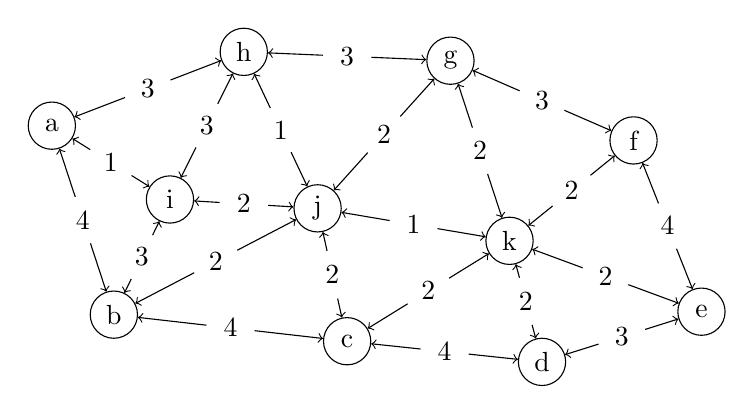
\begin{tikzpicture}[scale=0.750]
        \node[circle, draw, minimum size=0.6cm, inner sep=0pt] at (0.5* 0.0, 0.5* 8.5)  (a)    {a};
        \node[circle, draw, minimum size=0.6cm, inner sep=0pt] at (0.5* 2.1, 0.5* 2.1)  (b)    {b};
        \node[circle, draw, minimum size=0.6cm, inner sep=0pt] at (0.5* 10.0, 0.5* 1.2)  (c)    {c};
        \node[circle, draw, minimum size=0.6cm, inner sep=0pt] at (0.5* 16.6, 0.5* 0.5)  (d)    {d};
        \node[circle, draw, minimum size=0.6cm, inner sep=0pt] at (0.5* 22.0, 0.5* 2.2)  (e)    {e};
        \node[circle, draw, minimum size=0.6cm, inner sep=0pt] at (0.5* 19.7, 0.5* 8.0)  (f)    {f};
        \node[circle, draw, minimum size=0.6cm, inner sep=0pt] at (0.5* 13.5, 0.5* 10.7)  (g)    {g};
        \node[circle, draw, minimum size=0.6cm, inner sep=0pt] at (0.5* 6.5, 0.5* 11.0)  (h)    {h};
        \node[circle, draw, minimum size=0.6cm, inner sep=0pt] at (0.5* 4.0, 0.5* 6.0)  (i)    {i};
        \node[circle, draw, minimum size=0.6cm, inner sep=0pt] at (0.5* 9.0, 0.5* 5.7)  (j)    {j};
        \node[circle, draw, minimum size=0.6cm, inner sep=0pt] at (0.5* 15.5, 0.5* 4.6)  (k)    {k};

        \draw[<->]  (a) edge node[circle, fill=white] {4} (b);
        \draw[<->]  (a) edge node[circle, fill=white] {3} (h);
        \draw[<->]  (a) edge node[circle, fill=white] {1} (i);

        \draw[<->]  (b) edge node[circle, fill=white] {4} (c);
        \draw[<->]  (b) edge node[circle, fill=white] {3} (i);
        \draw[<->]  (b) edge node[circle, fill=white] {2} (j);

        \draw[<->]  (c) edge node[circle, fill=white] {4} (d);
        \draw[<->]  (c) edge node[circle, fill=white] {2} (j);
        \draw[<->]  (c) edge node[circle, fill=white] {2} (k);

        \draw[<->]  (d) edge node[circle, fill=white] {3} (e);
        \draw[<->]  (d) edge node[circle, fill=white] {2} (k);

        \draw[<->]  (e) edge node[circle, fill=white] {4} (f);
        \draw[<->]  (e) edge node[circle, fill=white] {2} (k);

        \draw[<->]  (f) edge node[circle, fill=white] {3} (g);
        \draw[<->]  (f) edge node[circle, fill=white] {2} (k);

        \draw[<->]  (g) edge node[circle, fill=white] {3} (h);
        \draw[<->]  (g) edge node[circle, fill=white] {2} (j);
        \draw[<->]  (g) edge node[circle, fill=white] {2} (k);

        \draw[<->]  (h) edge node[circle, fill=white] {3} (i);
        \draw[<->]  (h) edge node[circle, fill=white] {1} (j);

        \draw[<->]  (i) edge node[circle, fill=white] {2} (j);

        \draw[<->]  (j) edge node[circle, fill=white] {1} (k);
      \end{tikzpicture}
    }
    \caption{Vor der Kontraktion}
  \end{subfigure}
  \hfill
  \begin{subfigure}[b]{0.49\textwidth}
    \centering
    \resizebox{\textwidth}{!}{% <------ Don't forget this %
      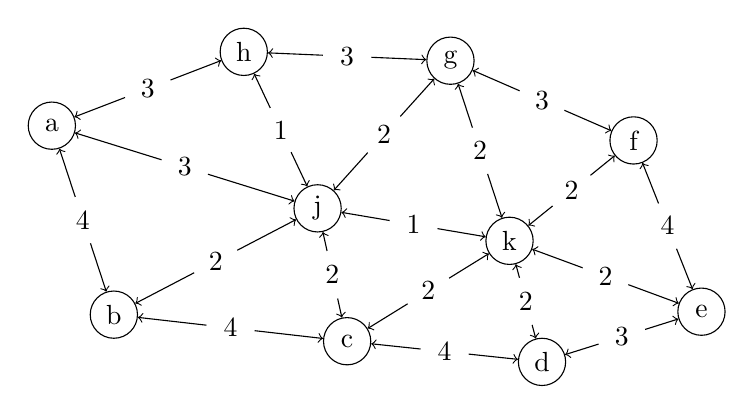
\begin{tikzpicture}[scale=0.750]
        % Nodes
        \node[circle, draw, minimum size=0.6cm, inner sep=0pt] at (0.5* 0.0, 0.5* 8.5)  (a)    {a};
        \node[circle, draw, minimum size=0.6cm, inner sep=0pt] at (0.5* 2.1, 0.5* 2.1)  (b)    {b};
        \node[circle, draw, minimum size=0.6cm, inner sep=0pt] at (0.5* 10.0, 0.5* 1.2)  (c)    {c};
        \node[circle, draw, minimum size=0.6cm, inner sep=0pt] at (0.5* 16.6, 0.5* 0.5)  (d)    {d};
        \node[circle, draw, minimum size=0.6cm, inner sep=0pt] at (0.5* 22.0, 0.5* 2.2)  (e)    {e};
        \node[circle, draw, minimum size=0.6cm, inner sep=0pt] at (0.5* 19.7, 0.5* 8.0)  (f)    {f};
        \node[circle, draw, minimum size=0.6cm, inner sep=0pt] at (0.5* 13.5, 0.5* 10.7)  (g)    {g};
        \node[circle, draw, minimum size=0.6cm, inner sep=0pt] at (0.5* 6.5, 0.5* 11.0)  (h)    {h};
        % \node[circle, draw, minimum size=0.6cm, inner sep=0pt] at (0.5* 4.0, 0.5* 6.0)  (i)    {i};
        \node[circle, draw, minimum size=0.6cm, inner sep=0pt] at (0.5* 9.0, 0.5* 5.7)  (j)    {j};
        \node[circle, draw, minimum size=0.6cm, inner sep=0pt] at (0.5* 15.5, 0.5* 4.6)  (k)    {k};

        \draw[<->]  (a) edge node[circle, fill=white] {4} (b);
        \draw[<->]  (a) edge node[circle, fill=white] {3} (h);
        \draw[<->]  (a) edge node[circle, fill=white] {3} (j);

        \draw[<->]  (b) edge node[circle, fill=white] {4} (c);
        \draw[<->]  (b) edge node[circle, fill=white] {2} (j);

        \draw[<->]  (c) edge node[circle, fill=white] {4} (d);
        \draw[<->]  (c) edge node[circle, fill=white] {2} (j);
        \draw[<->]  (c) edge node[circle, fill=white] {2} (k);

        \draw[<->]  (d) edge node[circle, fill=white] {3} (e);
        \draw[<->]  (d) edge node[circle, fill=white] {2} (k);

        \draw[<->]  (e) edge node[circle, fill=white] {4} (f);
        \draw[<->]  (e) edge node[circle, fill=white] {2} (k);

        \draw[<->]  (f) edge node[circle, fill=white] {3} (g);
        \draw[<->]  (f) edge node[circle, fill=white] {2} (k);

        \draw[<->]  (g) edge node[circle, fill=white] {3} (h);
        \draw[<->]  (g) edge node[circle, fill=white] {2} (j);
        \draw[<->]  (g) edge node[circle, fill=white] {2} (k);

        \draw[<->]  (h) edge node[circle, fill=white] {1} (j);

        \draw[<->]  (j) edge node[circle, fill=white] {1} (k);
      \end{tikzpicture}
    }
    \caption{Nach der Kontraktion}
  \end{subfigure}
  \caption{Kontraktion von $i$}
  \label{graphs:fig:example_contraction}
\end{figure}

Häufig wird die Kontraktionsbedingung abgeschwächt, indem dann eine Kante eingefügt wird, wenn der zu kontrahierende Knoten auf \emph{einem} kürzesten Pfad liegt.
Dazu kann eine normale Dijkstra-Suche verwendet werden: Ist die Länge einer potentiellen Abkürzung optimal, dann wird sie eingefügt.
Dies ist inbesondere dann effektiv, da die Suche, welche $v$ nicht begeht, den gesamten Graph absucht, wenn $(u, v, w)$ der einzige $u$-$w$-Pfad ist.
Weiter kann die Anzahl der Hops der Suche begrenzt werden.
Dadurch können jedoch auch unnötige Kanten eingefügt werden, die nicht unbedingt für die Erhaltung der kürzesten Pfad Distanz erforderlich sind.

\subsection{Graphen-Kontraktion}

Um die für die Beantwortung von Anfragen benötigte Datenstruktur, den \emph{Contracted-Graph}, zu erstellen, müssen alle Knoten eines Graphens kontrahiert werden, wobei die Kanten, die in jedem Schritt entfernt werden, gesammelt werden.
Hierbei hat die Reihenfolge, in der dies geschieht, einen großen Einfluss auf Perfomanz der nachfolgenden Kontraktionen und den mit der Methode erzielte Speedup.
Die Reihenfolge der Kontraktion wird durch eine \emph{vertex-to-level}-Funktion angegeben, die bijektiv ist und definiert als ${vtl} \colon V \to L$ mit $L \subset \mathbb{N}$, $\abs{L} = \abs{V}$ und $\max(L) = \abs{V}$.
Der Knoten mit dem niedrigsten \emph{Level} wird dabei zuerst kontrahiert.
Ihre Umkehrfunktion wird \emph{level-to-vertex}-Funktion genannt.

\begin{definition}[Contrated-Graph]
  Sei $G = (V, E)$ und $E'$ die durch die vollständige Kontraktion von $G$ erhalten Kanten mit der dazugehörigen vertex-to-level-Funktion ${vtl}$.

  Ein Contracted-Graph ist dann ein Tupel $C = (G_u, G_d)$. Der \emph{Upward-Graph} ist dabei $G_u = (V, E_u)$ mit $E_u = \{ (t, h) \mid (t, h) \in E' \colon {vtl}(h) > {vtl}(t) \}$, der \emph{Downward-Graph} ist $G_d = (V, E_d)$ mit $E_d = \{ (h, t) \mid (t, h) \in E' \colon {vtl}(h) < {vtl}(t) \}$.
\end{definition}

Der Name des Upward-Graphen ergibt sich daher, dass die Suche in einem Upward-Graph auf das Level bezogen nur \emph{aufwärts} geht.
In \cite{geisberger2008contraction} transponieren die Autoren die Kanten des Downward-Graphens nicht, daher geht ihre Suche \emph{abwärts}.
Die Transposition der Kanten ist hierbei nur ein Trick, damit auf dem Downward-Graphen wie auf dem Upward-Graphen \emph{vorwärts} gesucht wird.

Der entstandene Graph ist azyklisch, da er nur Kanten enthält, deren Kopf ein größeres Level als der dazugehörige Fuß hat.
Die Anzahl der in einer Breitensuche gefunden Knoten ist geringer als im Ursprungsgraph.
Diese Eigenschaften sorgen dafür, dass eine Suche in einem Upward-Graph kostengünstiger sein kann.
Die in einem Upward-Graph gefundenen kürzesten Pfade bilden eine obere Schranke für die tatsächlichen kürzesten Pfade; sie können jedoch auch länger sein als in $G$.
\autoref{graphs:fig:counterexample_optimal_Upward} zeigt ein Beispiel hierzu.
Die Knoten wurden in der Reihenfolge $c$, $d$, $a$, $b$ kontrahiert, wodurch der dazugehörige Upward-Graph entsteht.
Der optimale $c$-$a$-Pfad in $G$ hat die Distanz zwei, in $G_u$ hat er jedoch die Distanz drei.

\begin{figure}[ht]
  \centering
  \begin{subfigure}[b]{0.49\textwidth}
    \centering
    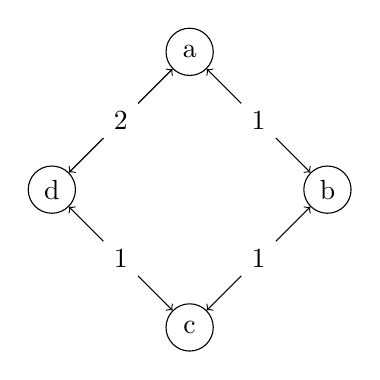
\begin{tikzpicture}
      \node[circle, draw, minimum size=0.6cm, inner sep=0pt] at (1.75*1.0, 1.75*2.0)  (a)    {a};
      \node[circle, draw, minimum size=0.6cm, inner sep=0pt] at (1.75*2.0, 1.75*1.0)  (b)    {b};
      \node[circle, draw, minimum size=0.6cm, inner sep=0pt] at (1.75*1.0, 1.75*0.0)  (c)    {c};
      \node[circle, draw, minimum size=0.6cm, inner sep=0pt] at (1.75*0.0, 1.75*1.0)  (d)    {d};

      \draw[<->]  (a) edge node[circle, fill=white] {1} (b);
      \draw[<->]  (b) edge node[circle, fill=white] {1} (c);
      \draw[<->]  (c) edge node[circle, fill=white] {1} (d);
      \draw[<->]  (d) edge node[circle, fill=white] {2} (a);
    \end{tikzpicture}
    \caption{Graph $G$}
  \end{subfigure}
  \hfill
  \begin{subfigure}[b]{0.49\textwidth}
    \centering
    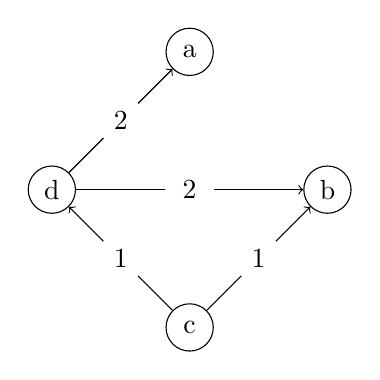
\begin{tikzpicture}
      \node[circle, draw, minimum size=0.6cm, inner sep=0pt] at (1.75*1.0, 1.75*2.0)  (a)    {a};
      \node[circle, draw, minimum size=0.6cm, inner sep=0pt] at (1.75*2.0, 1.75*1.0)  (b)    {b};
      \node[circle, draw, minimum size=0.6cm, inner sep=0pt] at (1.75*1.0, 1.75*0.0)  (c)    {c};
      \node[circle, draw, minimum size=0.6cm, inner sep=0pt] at (1.75*0.0, 1.75*1.0)  (d)    {d};

      \draw[->]  (c) edge node[circle, fill=white] {1} (b);
      \draw[->]  (c) edge node[circle, fill=white] {1} (d);
      \draw[->]  (d) edge node[circle, fill=white] {2} (b);
      \draw[->]  (d) edge node[circle, fill=white] {2} (a);
    \end{tikzpicture}
    \caption{Upward-Graph $G_u$ zu $G$}
  \end{subfigure}
  \caption{Gegenbeispiel optimale Kosten im $G_u$}
  \label{graphs:fig:counterexample_optimal_Upward}
\end{figure}

\subsection{Anfragen}

Die Suche eines kürzesten Pfades von $a$ nach $e$ auf dem Beispielgraph gestaltet sich nun wie folgt:
Auf $G_u$ wird eine Dijkstra-Suche von $a$ und auf $G_d$ eine Dijkstra-Suche von $e$ durchgeführt.
Aus den von beiden besuchten Knoten wird derjenige ausgewählt, der die niedrigste Summe beider Distanzen hat.
\autoref{fig:ch:beispiel_suche} zeigt einen auf diese Weise gefundenen Pfad auf dem Beispielgraph aus \autoref{graphs:fig:beispielgraph} von $a$ nach $e$.
Die Level der Knoten auf dem Pfad steigen von beiden Seiten an, bis sie den Treffpunkt-Knoten $j$ erreichen.
Die Kante $(a, j)$ ist hierbei eine Abkürzung, sie kürzt $i$ ab, was durch die gestrichelten Pfeile angedeutet wird.

\begin{figure}[ht]
  \centering
  \begin{tikzpicture}
    \node[circle, draw] at (0 * 1.5, -2 * 0.75)  (a)    {a};
    \node[circle, draw] at (1 * 1.5, -4 * 0.75)  (i)    {i};
    \node[circle, draw] at (2 * 1.5, -0 * 0.75)  (j)    {j};
    \node[circle, draw] at (3 * 1.5, -1 * 0.75)  (k)    {k};
    \node[circle, draw] at (4 * 1.5, -3 * 0.75)  (e)    {e};

    % draw axis
    \draw[->] (-1, -4 * 0.75) -- (-1, 0) node[above] {Level};

    \draw[->]  (a) -- (j);
    \draw[->]  (e) -- (k);
    \draw[->]  (k) -- (j);

    \draw[->, dotted]  (a) -- (i);
    \draw[->, dotted]  (i) -- (j);

  \end{tikzpicture}
  \caption{Beispiel einer Suche im Contrated Graph}
  \label{fig:ch:beispiel_suche}
\end{figure}

Algorithmus \ref{ch:query_simple} definiert dies formal.
Wie bei einer bidirektionalen Dijkstra-Suche wird der Pfad, sofern dieser existiert, aus den Teilpfaden beider Suchen erstellt.
Diese haben die Form $(u, \dotsc, t)$ bzw. $(v, \dotsc, t)$.
Um einen gültigen Pfad zu erstellen, muss $t$ aus einem dieser Teilpfade entfernt werden und der Pfad des Downward-Graphen umgekehrt werden.
Anschließend können beide Pfade verkettet werden und es entsteht ein Pfad auf $C$ der Form $(u, \dotsc, t, \dotsc, v)$.
Dieser Pfad muss aber kein Pfad auf $G$ sein, da er noch Abkürzungen enthalten kann.
In \autoref{ch:subsection:pfad_gewinnung} wird darauf eingegangen, wie diese entfernt werden können.

\begin{algorithm}[ht]
  \caption{Construction Hierarchies Query}
  \begin{algorithmic}[1]
    \Require Upward-Graph $G_u = (V, E_u)$, Downward-Graph $G_d = (V, E_d)$, Startknoten $s \in V$, Zielknoten $t \in V$
    \Ensure Treffknoten $m \in V \cup \{ {none} \}$, ${dist}_u$, ${pre}_u$, ${dist}_d$, ${pre}_d$
    \State ${dist}_u$, ${pre}_u$ $\leftarrow$ Dijkstra$(G_u, s)$
    \State ${dist}_d$, ${pre}_d$ $\leftarrow$ Dijkstra$(G_d, t)$

    \State
    \State $m \leftarrow {none}$
    \State $d \leftarrow \infty$
    \State
    Solche eine Abkürz
    \ForAll {$v \in V$}
    \If {${dist}_u(v) + {dist}_d(v) < d$}
    \State $m \leftarrow v$
    \State $d \leftarrow {dist}_u(v) + {dist}_d(v)$
    \EndIf
    \EndFor

    \State
    \State \Return $m$, ${dist}_u$, ${pre}_u$, ${dist}_d$, ${pre}_d$
  \end{algorithmic}
  \label{ch:query_simple}
\end{algorithm}

Die Korrektheit des Algorithmus ist nicht sofort ersichtlich, da nicht alle besuchten Knoten eine optimal Distanz haben sind und nur ein Teil aller Knoten besucht wird.
Der Beweis hierfür betrachtet einen kürzesten Pfad auf $G$ und argumentiert, warum dieser gefunden wird:

\begin{beweis}[Korrektheit Contracted-Graph Anfrage]\label{ch:proof:correct}
  Der Upward-Graph $G_u$ und der Downward-Graph $G_d$ enthalten nur Kanten, die mindestens so lang sind, wie der Abstand in $G$.
  Daher kann ein $s$-$t$-Pfad in $C$ nur dann gefunden werden, wenn auch in $G$ ein $s$-$t$-Pfad existiert.

  Nun ist zu zeigen, dass eine Suche auf $C$ die kürzesten Pfad Distanz in $G$ findet
  Sei ${sp}_G(s, t)$ der kürzeste Pfad auf $G$ der unter allen kürzesten Pfaden den Knoten $m$ mit dem höchsten Level enthält.
  Erstelle aus diesem Pfad $(s, \dotsc, t)$ zwei Pfade: $(s, \dotsc, m)$ und $(t, \dotsc, m)$.

  Betrachte den Teilpfad $(u, \dotsc, t)$ mit der Hop-Länge $n_u$.
  Aus diesem werden alle Knoten zwischen $u$ und $t$ entfernt, die ein kleineres Level als ihre Vorgänger haben.
  Dies wird so oft wiederholt, bis keine Knoten mehr entfernt werden.

  Betrachte den entstehenden Pfad als überlappende Tupel der Form $(v_{i}, v_{i + 1})$.
  Für diese gilt, dass ${vtl}(v_i) < {vtl}(v_{i + 1})$, da wir uns im Teilpfad des Upward-Graphens befinden.
  Die Knoten-Kontraktion erhält den Abstand der übrigen Knoten, also gab es zum Zeitpunkt der Kontraktion von $v_i$ einen optimalen Pfad von $v_i$ zu $v_{i + 1}$.
  Alle Knoten, die ursprünglich zwischen ihnen lagen und entfernt wuren, haben ein kleineres Level als $v_i$, waren also zum Zeitpunkt der Kontraktion von $v_i$ bereits Kontraktiert.
  Also gab es vor der Kontraktion von $v_i$ eine direkte Kante zu $v_{i + 1}$, diese wurde gesammelt und dazu benutzt den Upward-Graphen zu bauen.
  Daher wird $v_{i + 1}$ von $v_i$ aus gefunden.
  Da dies für alle überlappenden Tupel gilt, wird $t$ von $u$ aus mit optimalen Abstand gefunden.

  Analog wird für den Teilpfad $(t, \dotsc, m)$ im Downward-Graphen argumentiert.
  \qed
\end{beweis}

\subsection{Erstellung des Pfades}\label{ch:subsection:pfad_gewinnung}

Der in $C$ gefundene Pfad kann bisher noch Abkürzungen enthalten.
Damit der Pfad auch auf $G$ gültig ist, müssen diese ersetzt werden.
Hierfür ist eine Funktion notwendig, welche diese ersetzt.

Solche eine Abkürzungsfunktion kann etwa durch eine HashMap implementiert werden.
Da die ${vtl}$-Funktion bijektiv ist, gilt für alle Knoten $u, v \in V$, $u \neq v$ immer entweder ${vtl}(u) < {vtl}(v)$ oder ${vtl}(u) > {vtl}(v)$.
Daher reicht es für die Ersetzung der Abkürzungen in Pfaden in $C$ \emph{eine} HashMap zu benutzen, da keine Kollisionen zwischen Abkürzungen des Upward- und des Downward-Graphen entstehen können.

\begin{figure}[ht]
  \centering
  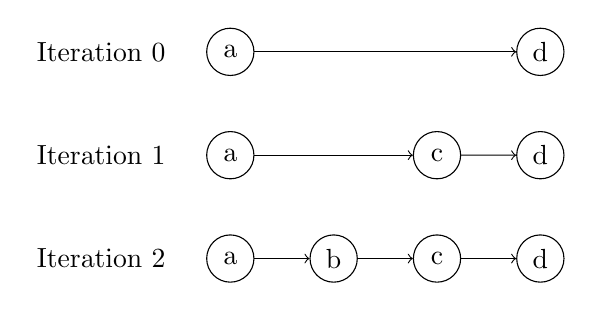
\begin{tikzpicture}[scale=0.75]
    \node[align=left] at (1.75*-1.25,1.75*2) {Iteration 0};
    \node[circle, draw, minimum size=0.6cm, inner sep=0pt] at (1.75*0.0, 1.75*2.0)  (a_0)    {a};
    \node[circle, draw, minimum size=0.6cm, inner sep=0pt] at (1.75*3.0, 1.75*2.0)  (d_0)    {d};
    \draw[->]  (a_0) edge node {} (d_0);

    \node[align=left] at (1.75*-1.25,1.75*1) {Iteration 1};
    \node[circle, draw, minimum size=0.6cm, inner sep=0pt] at (1.75*0.0, 1.75*1.0)  (a_1)    {a};
    \node[circle, draw, minimum size=0.6cm, inner sep=0pt] at (1.75*2.0, 1.75*1.0)  (c_1)    {c};
    \node[circle, draw, minimum size=0.6cm, inner sep=0pt] at (1.75*3.0, 1.75*1.0)  (d_1)    {d};
    \draw[->]  (a_1) edge node {} (c_1);
    \draw[->]  (c_1) edge node {} (d_1);

    \node[align=left] at (1.75*-1.25,1.75*0) {Iteration 2};
    \node[circle, draw, minimum size=0.6cm, inner sep=0pt] at (1.75*0.0, 1.75*0.0)  (a_2)    {a};
    \node[circle, draw, minimum size=0.6cm, inner sep=0pt] at (1.75*1.0, 1.75*0.0)  (b_2)    {b};
    \node[circle, draw, minimum size=0.6cm, inner sep=0pt] at (1.75*2.0, 1.75*0.0)  (c_2)    {c};
    \node[circle, draw, minimum size=0.6cm, inner sep=0pt] at (1.75*3.0, 1.75*0.0)  (d_2)    {d};
    \draw[->]  (a_2) edge node {} (b_2);
    \draw[->]  (b_2) edge node {} (c_2);
    \draw[->]  (c_2) edge node {} (d_2);
  \end{tikzpicture}
  \caption{Beispiel des iterativen Ersetzen von Abkürzungen}
\end{figure}

Um diese Funktion zu erhalten, müssen die Abkürzungen, welche beim Kontrahieren des Graphens eingefügt werden, mitsamt dem übersprungenen Knoten gesammelt werden.
Einen möglichen Algorithmus, welcher Abkürzungen in einem Pfad ersetzt, ist in Algorithmus \ref{ch:alg:shortcut_replacement} zu sehen.
Der Algorithmus betrachtet den Pfad mit Abkürzungen als Stapel und bearbeitet jeweils nur die beiden obersten Knoten, da das Einfügen in ein Array an einer bestimmten Stelle rechenintensiv ist.

\begin{algorithm}[ht]
  \caption{Shortcut replacement}
  \begin{algorithmic}[1]
    \Require Pfad $p$ mit Abkürzungen, Abkürzungungsfunktion $S \colon V \times V \to V \cup \{ {none} \}$
    \Ensure Pfad $p'$ ohne Shortcuts

    \If {$\text{len}(p) == 1$}
    \State \Return $p$
    \EndIf
    \State

    \State $p' \leftarrow ()$
    \State

    \While {$\text{len}(p) >= 2$}
    \State $w \leftarrow \text{pop}(p)$
    \State $u \leftarrow \text{pop}(p)$
    \State $v \leftarrow S((u, w))$
    \State

    \If {$v \neq none$}
    \State $\text{push}(p, u)$
    \State $\text{push}(p, v)$
    \State $\text{push}(p, w)$
    \Else
    \State $\text{push}(p, u)$
    \State $\text{push}(p', w)$
    \EndIf
    \EndWhile

    \State
    \State $p' \leftarrow \text{reversed}(p')$

    \State
    \State \Return $p'$
  \end{algorithmic}
  \label{ch:alg:shortcut_replacement}
\end{algorithm}

\subsection{Early stop}

Der Algorithmus \ref{ch:query_simple} ist von theoretischer Bedeutung.
Implementierungen ähneln der bidirektionalen Dijkstra-Suche, es werden also abwechselnd Knoten der Upward-Suche und der Downward-Suche expandiert.
Die Expansion einer Suchrichtung kann dabei gestoppt werden, wenn die kleinste Distanz der Vorwärtswarteschlange größer als die bisherige kleinste Treffpunkt-Distanz ist.
Wenn beide Suchen gestoppt sind, ist ein vorhandener kürzester Pfad gefunden worden.

\subsection{Stall-on-demand}

Wie \autoref{graphs:fig:counterexample_optimal_Upward} zeigt, sind manche der im Upward- und Downward-Graphen gefunden Distanzen nicht optimal.
Für das Finden einen kürzesten Pfades sind jedoch nur die Knoten interessant, deren Distanz optimal ist.
Mit der von \cite{schultes2007dynamic} vorgestellten Methode \emph{stall-on-demand} ist es möglich, den Suchraum der beiden Teilsuchen zu verkleinern.
Hierfür wird die Expansion eines Knotens abgebrochen, wenn er durch eine Kante des jeweils anderen Graphen günstiger erreicht werden kann.

\begin{definition}[stall-on-demand]
  Sei $C = (G_u, G_d)$ ein Contracted-Graph mit $G_u = (V, E_u)$ und $G_d = (V, E_d)$.
  Der Knoten $u \in V$ hat keine optimale Distanz in der Dijkstra-Suche von $s$ in $G_u$, wenn zum Zeitpunkt seiner Expansion es eine Kante $(u, v, d) \in E_d$, $v \in V$, $d \in \mathbb{R}$ gibt mit ${dist}(v) + d < {dist}(u)$.
  Die Expansion von $u$ kann dann abgebrochen werden, die aus $u$ ausgehenden Kanten müssen nicht betrachtet werden.
  Gleiches gilt analog für $G_d$.
\end{definition}

Betrachten wird dies an dem Beispiel in \autoref{fig:ch:stall_example}.
Wir befinden uns in der Suche des Upward-Graphens
Die blauen Kanten sind dabei Kanten der Upward-Suche, die rote Kante eine von $u$ ausgehende Downward-Kante.
Bisher wurde $v$ in der Upward-Suche mit einer Distanz von eins expandiert, als Nächstes soll $u$ expandiert werden.
$u$ hat die Distanz drei in der Upward-Suche, kann aber durch die Verwendung der Upward-Kante mit der Distanz zwei erreicht werden, also ist die Distanz drei nicht optimal und von $u$ ausgehenden Kanten müssen nicht relaxiert werden.

\begin{figure}
  \centering
  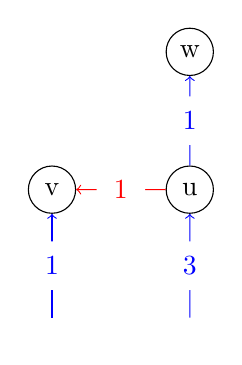
\begin{tikzpicture}[scale=1.75]
    \node[circle, draw, minimum size=0.6cm, inner sep=0pt] at (0, 2)  (v)    {v};
    \node[circle, draw, minimum size=0.6cm, inner sep=0pt] at (1, 2)  (u)    {u};
    \node[circle, draw, minimum size=0.6cm, inner sep=0pt] at (1, 3)  (w)    {w};

    \node[] at (0, 1)  (uv)    {};
    \node[] at (1, 1)  (uu)    {};

    \draw[->,blue]  (u) edge node[circle, fill=white] {1} (w);

    \draw[->,red]  (u) edge node[circle, fill=white] {1} (v);

    \draw[->,blue]  (uv) edge node[circle, fill=white] {1} (v);
    \draw[->,blue]  (uu) edge node[circle, fill=white] {3} (u);
  \end{tikzpicture}
  \caption{Beispiel stall-on-demand}
  \label{fig:ch:stall_example}
\end{figure}

\subsection{Erstellung}

Ein Contracted-Graph wird durch die vollständige Kontraktion eines Graphens erstellt.
Die Reihenfolge, in der die Knoten kontrahiert werden, kann dabei im Voraus feststehen oder es wird iterativ der jeweils \emph{unwichtigste} Knoten kontrahiert.
An den Prozess der Erstellung können mehrere Kriterien angelegt werden: So kann die Geschwindigkeit der Erstellung, die Geschwindigkeit der Anfragen oder die Anzahl der hinzugefügten Abkürzungen minimiert werden.

\subsubsection{Top-Down}
Bei der Top-Down-Kontraktion ist die level-to-vertex-Funktion ${ltv}$ vorgegeben.
Die Knoten werden in Reihenfolge ihres Levels kontrahiert, wobei mit dem niedrigsten Level begonnen wird.
Diese Herangehensweise bietet einerseits die Möglichkeit dafür eine optimale Reihenfolge anzuwenden, wobei diese für hinreichend große Graphen nur schwer bestimmbar ist.

\paragraph{Sortiert nach Grad}
Die Knoten werden nach ihrem Grad sortiert, wobei die kleinsten Grade zuerst kontrahiert werden.
Die Überlegung dahinter ist, dass Knoten mit vielen Nachbarn auch viele neue Kanten einfügen können, was vermieden werden soll.
Nach größtem Grad ist vielleicht auch spannend.

\paragraph{Sortiert durch Hitting-Set}
Es wird über eine möglichst große Anzahl an Pfaden ein Hitting-Set gebildet, die Knoten des Hitting-Sets werden dann nach der Anzahl ihrer Hits sortiert.
Die Knoten die nicht Teil des Hitting-Set sind, werden anschließend die unteren Level zugewiesen, wobei diese wiederum nach einer Metrik sortiert werden können, wie etwa dem Grad.

\subsubsection{Bottom-Up}

Bei der Bottom-Up-Kontraktion wird die vertex-to-level-Funktion ${vtl}$ während der Kontraktion erstellt.
Dafür wird mit einer Heuristik der jeweils \emph{unwichtigste} Knoten aus einer Prioritätswarteschlange ausgewählt und kontrahiert.
Ein unwichtiger Knoten hat hierbei einen niedrigen Heuristikwert.
Die in der Praxis am meistverwendeten Heuristiken beinhalten die \emph{Kanten-Differenz}, ziehen jedoch zumeist auch noch weitere Informationen mit ein.
Sie gibt an, wie sich die Anzahl der Kanten im gesamten Graph durch die Kontraktion verändert.
Sie wird gebildet, indem die Anzahl der neu hinzugefügten Kanten von der Anzahl der entfernten Kanten subtrahiert wird.
Die Kontraktion eines Knotens kann dabei die Heuristikwerte anderer Knoten verändern.
Damit jedes Mal der Knoten mit dem niedrigsten Heuristikwert ausgewählt wird, müssen nach jeder Kontraktion alle Heuristikwerte neuberechnet werden.
Dies ist im Allgemeinen jedoch zu teuer, weshalb in der Praxis sich zwei Methoden als effektiv erwiesen haben:

Beim \emph{Lazy-Popping} wird davon ausgegangen, dass ein Knoten nur wichtiger werden kann.
Aus der Warteschlange wird ein Knoten entnommen und geprüft, ob sein Heuristikwert gewachsen ist.
Wenn er gewachsen ist, dann wird er zurück in die Warteschlange geschoben, wenn nicht, dann wird er kontraktiert.
Dies wird wiederholt, bis schließlich ein Knoten gefunden wird.
Beim \emph{Neighbor-Update} werden nach der Kontraktion eines Knotens die Heuristikwerte der Nachbarn aktualisiert.

Um die zu einem Contracted-Graph dazugehörige Abkürzungsfunktion zu erhalten, muss während der Kontraktion des Graphens eine Liste der Abkürzungen erstellt werden.
Wird die im vorherigen Absatz erwähnte abgeschwächte Bedingung verwendet, muss darauf geachtet werden, dass sich die Abkürzung zweier Knoten während der Kontraktion des Graphens mehrmals ändern kann, nur die letzte, beste Abkürzung darf dann gespeichert werden.

\section{Hierachical Hub Labeling}\label{chapter:hl}

Die Contracted-Graph-Anfrage ohne Stopbedingung erstellt jeweils den vollen Suchbaum für den Start und Zielknoten und sucht aus den expandierten Knoten beider Suchen den Knoten mit geringster Summe der Distanzen in beiden Suchen.
Die Idee des Labels ist es, den Suchbaum des Upward- bzw. Downward-Graphen zu speichern, eine $s$-$t$-Anfrage ist dann nur noch der Vergleich zweier Labels.
In der in \cite{abraham2011hub} vorgestellten Terminologie wird das Label des Upward-Graphen \emph{Forward-Label} und das des Downward-Graphen \emph{Backward-Label} genannt.
Ein kürzester Pfad wird gefunden, in dem der Knoten mit der geringsten Summe der Distanzen des Forward und Backward-Labels gefunden wird.

\begin{definition}[Hub Graph]
  Sei $G = (V, E)$.
  Ein \emph{Hub Graph} ist $H = (L_f, L_b)$ und es gilt:
  Die Forward-Label-Funktion $L_f \colon V \to V \times \mathbb{R}^+_0$ weist jedem Knoten ein Forward-Label zu.
  Sei $L_f (u)$ das Forward-Label des Knotens $u \in V$, dann gibt es für jeden Knoten $v \in V$ höchstens ein $(v, d) \in L_f (u)$ und es gilt $d \geq {spd}_G(u, v)$.
  Ein Backward-Label ist ein Forward-Label des Umkehrgraphens $G^T$.

  Zusammen erfüllen die Forward-Label und die Backward-Label die Abdeckungseigenschaft:
  Für jedes Knotenpaar $s, t \in V$ für die es einen kürzesten $s$-$t$ Pfad gibt, gibt es einen Knoten $m \in V$ mit $(m, d_f) \in L_f (s)$, $(m, d_r) \in L_r$ und $d_f + d_r = {spd}_G (s, t)$.
\end{definition}

Die Definition der Label ähnelt bereits dem Beweis der Korrektheit der Contracted-Graph Query, bei diesem wurde ebenfalls mit dem Treffpunktknoten $m$ argumentiert.
Aus einem Contracted-Graphen lässt sich ein Hub Graph bauen, indem der Suchbaum des Upward-Graphen als Forward-Label und der des Downward-Graphen als Backward-Label betrachtet wird, denn die Suchbäume treffen sich im Knoten mit dem höchsten Level mit optimalem Abstand.
Die Erstellung kann auf zwei Wegen geschehen, durch eine Dijkstra-Suche im Upward- bzw. Downward-Graphen pro Knoten oder durch \emph{Merging}.
Diese so erstelten Labels sind hierarchisch: Es gibt eine Ordnung der Knoten (die vertex-to-level-Funktion), so dass das Forward und das Backward-Label eines Knotens $u$ nur Knoten $h$ mit höherer Ordnung enthält.
Es sind auch Label möglich, die diese Eigenschaft nicht erfüllen, weiter können solche für manche Graphen deutlich kleiner sein, als hierarchische.\cite{goldberg2013separating}

\subsubsection{Anfrage}

Sei $H = (L_f, L_b)$ ein Hub-Graph.
Algorithmus \ref{hl:alg:query} zeigt, wie wenige Schritte dafür notwendig sind, eine kürzeste Pfad Distanz in $H$ zu finden, nur noch das Finden des Knotens mit der geringsten Summe der Distanzen ist dafür erforderlich.
Da die Labels den Suchbäumen der Upward- bzw. Downward-Suche entsprechen, ist die Korrektheit der Hub-Graph-Anfrage durch die Korrektheit der Contracted-Graph-Anfrage gegeben.

\begin{algorithm}[ht]
  \caption{Hub-Label-Anfrage}
  \begin{algorithmic}[1]
    \Require Forward-Label-Funktion $L_f$, Backward-Label-Funktion $L_b$, Startknoten $s \in V$, Zielknoten $t \in V$
    \Ensure Treffknoten $m \in V \cup \{ {none} \}$, ${dist}_u$
    \State $l_s \leftarrow L_f (s)$
    \State $l_t \leftarrow L_b (t)$

    \State
    \State $m \leftarrow {none}$
    \State $d \leftarrow \infty$

    \ForAll {$v \in V \colon (v, d_f) \in l_s \land (v, d_r) \in l_t$}
    \If {$d_f + d_r < d$}
    \State $d \leftarrow d_f + d_r$
    \State $m \leftarrow v$
    \EndIf
    \EndFor

    \State
    \State \Return $m$, $d$
  \end{algorithmic}
  \label{hl:alg:query}
\end{algorithm}

\subsection{Pfaderstellung}

Nachdem ein Treffpunkt-Knoten $m$ gefunden wurde, sind noch zusätzliche Informationen notwendig, um einen Pfad in $G$ erstellen zu können, denn zuerst muss ein Pfad in $C$ erstellt werden und anschließend die Abkürzungen ersetzt werden.
Dafür muss für jeden Knoten in einem Label sein Vorgänger, falls vorhanden, bekannt sein.
Dafür wird die Definition des Label von einer Teilmenge von $V \times \mathbb{R}$ erweitert auf eine Teilmenge von $V \times \mathbb{R} \times (V \cup \{ none \}) $, der zusätzliche Knoten speichert hierbei den Vorgängern.
Für das Erstellen eines Pfades springt man, beginnend vom Treffpunkt-Knoten durch alle Vorgänger, bis es keinen Vorgänger mehr gibt.
Durch das Ersetzen der Abkürzungen, etwa mit dem Algorithmus \ref{ch:alg:shortcut_replacement}, erhält man so einen gültigen Pfad auf $G$.

\subsection{Datenstruktur}

Gibt es eine Totalordnung der Knoten, dann lässt sich durch eine geschickte Wahl der Datenstruktur zur Speicherung eines Labels der Knoten mit der geringsten Summe der Distanzen in linearer Zeit zur Größe der Label finden:
Labels sind dann eine Liste und deren Einträge nach dem Knoten sortiert.
Ähnlich wie bei Merge Sort werden dabei die Einträge paarweise verglichen, wobei der Index des Labels mit dem jeweils kleineren Element inkrementiert wird.
Dadurch ist garantiert, dass alle Knoten, welche in beiden Labeln vorhanden sind, Zeitgleich betrachtet werden und falls diese einen aktuell besten Treffpunkt-Knoten bilden, diese Information gespeichert werden kann.

Um das Finden der Vorgänger effizienter zu machen, wird nicht der Vorgänger selbst gespeichert, sondern sein Index im Label.
\autoref{ch:fig:label} zeigt ein Label solcher Art.

\begin{figure}[ht]
  \centering
  \begin{tabular}{@{}llllll@{}}
    \toprule
    Index           &  & 0   & 1   & 2   & 2 \\ \midrule
    Vertex          &  & $e$ & $j$ & $k$ &   \\
    Distanz         &  & 0   & 3   & 2   &   \\
    Vorgänger Index &  & -   & 2   & 0   &   \\ \bottomrule
  \end{tabular}
  \caption{Beispiel eines Labels}
  \label{ch:fig:label}
\end{figure}

\subsection{Erstellung}

Da die Label den expandierten Knoten im Suchbaum des Upward-bzw. Downward-Graph entspricht, können diese naiv dadurch gebildet werden, dass pro Knoten der entsprechende Suchbaum mit einer Dijkstra-Suche erstellt wird und die gefundenen Knoten entsprechend sortiert werden.
Dies lässt sich gut parallelisieren, jedoch ist das \emph{Merging} meist effizienter.

\subsubsection{Merging}

Für jeden Knoten des Graphens $G$ wird ein Label vorbereitet, das zu Beginn nur den Knoten selbst enthält.
Danach werden die Label in der Reihenfolge der Level, von groß zu klein, wie folgt erstellt:
Pro Knoten werden die ausgehenden Kanten des Downward bzw. Upward-Graphens betrachtet.
Die Köpfe dieser Kanten haben ein höheres Level als der Knoten selbst, daher existieren ihren Label bereits.
Sie werden gemerged, indem sie zusammen ein neues Label bilden und Duplikate mit größerer Distanz entfernt werden.
Dies erstellt ebenfalls die benötigten Suchbäume des Upward- bzw. Downward-Graph.

\todo{Bild}

\subsubsection{Pruning}

Die erstellten Labels enthalten bisher noch Knoten mit nicht-optimaler Distanz in $G$ (siehe \autoref{graphs:fig:counterexample_optimal_Upward}), was einerseits den Speicherbedarf der  Label als auch die Abfrage Zeiten erhöht.
Die Einträge mit nicht-optimaler Distanz können dabei entfernt werden, indem die erstellten Hub Label selbst dafür benutzt werden, die Einträge mit nicht-optimaler Distanz zu identifizieren.
Diese nicht-optimale Einträge können aus dem Label entfernt werden.
Beim Merging kann dies auch bereits während der Erstellung geschehen, da die Labels von Knoten mit höherem Level bereits existieren.
